\section{Contexte}

\subsection{L'arnaque du serrurier}

% TODO le slide qui affiche la subsec = inutile

\long\def\mecnocol{
    \draw[ultra thick]
              (0, 0)
        -- ++ (1, -2)
        -- ++ (1, 0)
        -- ++ (-1, 3)
        -- ++ (1, -1)
        -- ++ (1, 1)
        -- ++ (-2, 1)
        -- ++ (0, 1)
        -- ++ (-2, 0)
        -- ++ (0, -1)
        -- ++ (-2, -1)
        -- ++ (1, -1)
        -- ++ (1, 1)
        -- ++ (-1, -3)
        -- ++ (1, 0)
        -- cycle;
}

\long\def\mec{
    \draw[fill=MellonGreen]
              (0, 0)
        -- ++ (1, -2)
        -- ++ (1, 0)
        -- ++ (-1, 3)
        -- ++ (1, -1)
        -- ++ (1, 1)
        -- ++ (-2, 1)
        -- ++ (0, 1)
        -- ++ (-2, 0)
        -- ++ (0, -1)
        -- ++ (-2, -1)
        -- ++ (1, -1)
        -- ++ (1, 1)
        -- ++ (-1, -3)
        -- ++ (1, 0)
        -- cycle;
    \mecnocol{}
}

\long\def\portepoigneefermee{
    \draw[ultra thick]
           (3.5, 2)
        -- ++ (0.6, -0.24)
        circle(0.1);
}

\long\def\portepoigneeouverte{
    \draw[ultra thick]
           (2.5, 3.6)
        -- ++ (0.6, 0.14)
        circle(0.1);
}

\long\def\portefermee#1{
    \draw[fill=#1]
              (0, 0)
        -- ++ (5, -2)
        -- ++ (0, 8)
        -- ++ (-5, 2)
        -- cycle;

    \portepoigneefermee{}
}
\long\def\portecadre{
    \draw[ultra thick]
              (0, 0)
        -- ++ (5, -2)
        -- ++ (0, 8)
        -- ++ (-5, 2)
        -- cycle;
}

\long\def\porte#1{
    \portefermee{#1}
    \portecadre{}
    \portepoigneefermee{}
}

\long\def\porteouv#1{
    \portecadre{}
    \draw[ultra thick, fill=#1]
                (0, 0)
           -- ++(4, 1)
           -- ++(0, 5.4)
           -- ++(-4, 1.6)
           -- (0, 0);
    \portepoigneeouverte{}
}

\long\def\serrurier{
    \mecnocol{}
    \node at (0, 1.2) {S};

    \path (0, 0)
        -- ++ (5, -2)
        -- ++ (0, 8)
        -- ++ (-5, 2)
        -- cycle;
}

\begin{frame}{L'arnaque du serrurier}

    \centering
    $
    \vcenter{\hbox{
    
\begin{tikzpicture}
        [scale=0.2]
        \serrurier{}
    \end{tikzpicture}
    }}
    +
    \vcenter{\hbox{
    \begin{tikzpicture}
        [scale=0.2]
        \only<1>{ \porte{MellonGreen} }
        \only<2>{ \porte{MellonPink} }
        \mec{}
    \end{tikzpicture}
    }}
    =
    \vcenter{\hbox{
    \begin{tikzpicture}
        [scale=0.2]
        \only<1>{ \porteouv{MellonGreen} }
        \only<2>{ \porteouv{MellonPink} }
        \mec{}
    \end{tikzpicture}
    }}
    $

\begin{itemize}
    \item J'appelle un serrurier
    \item Je l'attends devant \only<1>{\textbf{chez moi}}\only<2>{\textbf{chez mon voisin}}
    \item Il ouvre \only<1>{\textbf{ma porte}}\only<2>{\textbf{sa porte}}
    \item Je rentre \only<1>{\textbf{chez moi}}\only<2>{\textbf{chez mon voisin}}
\end{itemize}
\end{frame}

%\begin{frame}{L'arnaque du serrurier -- conclusion}
%
%\begin{itemize}
%\item Problème de confiance
%\item il ne doit pas appliquer ses droits
%\item …mais ceux de l'appelant
%\item Il doit vérifier que j'ai bien les droits sur la maison
%\end{itemize}
%
%\end{frame}

\subsection{Isolation entre utilisateur et noyau}

% TODO code couleur ici

\begin{frame}{Utilisateur et noyau}
    \centering
    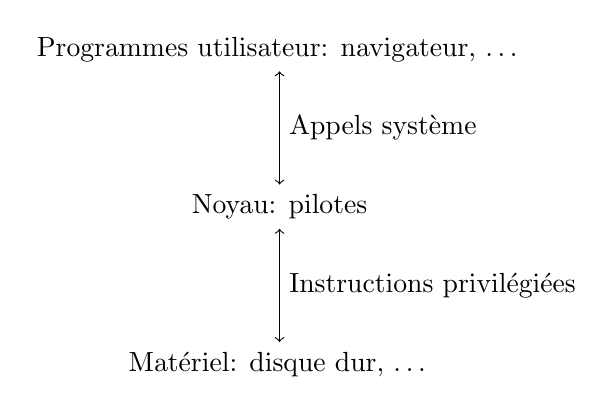
\begin{tikzpicture}
        [node distance=2cm]
        \node (U) {Programmes utilisateur: navigateur, …};
        \node[below of=U] (K) {Noyau: pilotes};
        \node[below of=K] (H) {Matériel: disque dur, …};
        \draw[<->] (U) -- node [auto] {Appels système} (K);
        \draw[<->] (K) -- node [auto] {Instructions privilégiées} (H);
    \end{tikzpicture}
\end{frame}

% Memory zone
%
% #1 - start
% #2 - end
% #3 - color
\newcommand{\mzone}[3]{
  \path[#3] (#1,0) rectangle (#2,1);
}

% Address label
%
% #1 - x position
% #2 - text
\newcommand{\alabel}[2]{
  \path (#1,1) -- ++(0,0.3) node [pos=1] {\small \tt #2};
}
\newcommand{\addrlabel}[2]{
  \draw[<-] (#1,-0.1) -- ++(0,-0.3) node [auto,pos=1] {\small \tt #2};
  \draw[pattern=north east lines] (#1,0) rectangle ++(0.2,1);
}
\long\def\memzones{

  \mzone{0}{6}{user}
  % exec
  %\mzone{0.5}{1}{user}

  %% lib
  %\mzone{2.5}{3.2}{user}

  %% stack
  %\mzone{3.7}{4}{user}

  %% stack
  %\mzone{5}{5.5}{user}

  % kernel
  \mzone{6}{8}{kernel}

  % contour
  \draw (0,0) rectangle (8,1);

  \alabel{0}{0}
  \alabel{6}{3 Go}
  \alabel{8}{4 Go}

}

%\begin{frame}[fragile]{Séparation}
%\begin{tikzpicture}
%  [user/.style={fill=MellonGreen}
%  ,kernel/.style={fill=MellonPink}
%  ]
%
%  \memzones{}
%
%  \node at (2, -0.7) {Programme};
%  \node at (7, -0.7) {Noyau};
%
%  \draw[>=triangle 45,<->,ultra thick] (3.8, -0.7) -- node[auto] {Appels système} ++(2, 0);
%  \draw[>=triangle 45,<->,ultra thick] (7, -1) -- node[auto,swap] {Instructions
%  privilégiées} ++(0, -1) node (Htop) {};
%
%  \path (Htop) -- ++(-1,-1) node (Htopleft) {};
%  \draw (Htopleft) rectangle ++(2, -2);
%
%  \foreach \x in {0,...,9} {
%      \draw ($ (Htopleft) + (0.1 + 0.2*\x,  0) $) -- ++(0,  0.3);
%      \draw ($ (Htopleft) + (0.1 + 0.2*\x, -2) $) -- ++(0, -0.3);
%      \draw ($ (Htopleft) + (0, -0.2*\x - 0.1) $) -- ++(-0.3, 0);
%      \draw ($ (Htopleft) + (2, -0.2*\x - 0.1) $) -- ++( 0.3, 0);
%   }
%
%  \path (Htop) -- ++(0, -2) node { Matériel };
%
%\end{tikzpicture}
%\end{frame}

\begin{frame}{Mémoire utilisateur et noyau}
\centering
\begin{tikzpicture}
  [user/.style={fill=MellonGreen}
  ,kernel/.style={fill=MellonPink}
  ]

  \memzones{}

  \node at (3, -1) (LU) {\parbox{3cm}{\centering Programmes utilisateur}};
  \node at (7, -1) (LK) {Noyau};

  \node[minimum width=6cm] at (3, 0) (MU) {};
  \node[minimum width=2cm] at (7, 0) (MK) {};

  \node[below=2cm of LK] (HW) {Matériel};

  \draw[<->] (LU) -- (MU);
  \draw[<->] (LK) -- (MU);
  \draw[<->] (LK) -- (MK);
  \draw[<->] (LU) -- node[auto, swap] {\parbox{2cm}{\centering Appels système}} (LK);
  \draw[<->] (LK) -- node[auto]       {\parbox{2cm}{\centering Instructions privilégiées}} (HW);

\end{tikzpicture}
\end{frame}

\begin{frame}{Utilisation correcte d'un appel système}
\centering
    \insertcode{gettimeofday.c}

\begin{tikzpicture}
  [user/.style={fill=MellonGreen}
  ,kernel/.style={fill=MellonPink}
  ]

  \memzones{}
  \addrlabel{2.7}{ptv}
\end{tikzpicture}
\end{frame}

\begin{frame}{Utilisation détournée d'un appel système}
\centering
    \insertcode{gettimeofday-bad.c}

\begin{tikzpicture}
  [user/.style={fill=MellonGreen}
  ,kernel/.style={fill=MellonPink}
  ]

  \memzones{}
  \addrlabel{6.7}{ptv}
  
    % TODO pourquoi est-ce un pb
\end{tikzpicture}
\end{frame}

\def\ssout{\bgroup
 \markoverwith{\lower-0.2ex\hbox
 {\kern-.03em\vbox{\hrule width.2em\kern0.45ex\hrule}\kern-.03em}}%
 \ULon}
\MakeRobust\dout

\begin{frame}{Problème des pointeurs dans les appels système}

\begin{minipage}{0.65\textwidth}
\begin{itemize}
    \item La copie simple n'est pas suffisante:\newline il faut vérifier tous les pointeurs
    \item 2 propriétés:
    \begin{itemize}
        \item Qui contrôle le pointeur?
        \item Dans quelle plage se trouve sa valeur?
    \end{itemize}
    \item Invariant: les pointeurs contrôlés par l'utilisateur pointent dans la
        mémoire utilisateur
    \item Fonctions non sûres: \texttt{memcpy}, \texttt{strcpy}
    \item Fonctions sûres: \texttt{copy\_from\_user}, \texttt{copy\_to\_user}
\end{itemize}
\end{minipage}
\begin{minipage}{0.25\textwidth}
    \begin{tikzpicture}
        [ lbl/.style={ auto
                     }
        ]
        \draw[fill=MellonGreen] (0, 0) rectangle (-1.7, 6);
        \draw[fill=MellonPink] (0, 0) rectangle (1.7, 6);

        \draw[->] (-1, 5)  to[bend left]  node[lbl] {\texttt{copy\_from\_user}} ++ (2, 0);
        \draw[->] (-1, 4)  to[bend left]  node[lbl] (MB1) {\texttt{memcpy}} ++ (2, 0);
        \draw[<-] (-1, 2)  to[bend right] node[lbl,swap] {\texttt{copy\_to\_user}} ++ (2, 0);
        \draw[<-] (-1, 1)  to[bend right] node[lbl,swap] (MB2) {\texttt{memcpy}} ++ (2, 0);
        \draw[<-] (0.2, 2.5) to[bend right] node[lbl,swap] {\texttt{memcpy}} ++ (0, 1);

        \foreach \N in {MB1,MB2}
        \draw[thick] ($ (\N.east) + (0, 0.5mm) $)
                  -- ($ (\N.west) + (0, 0.5mm) $);
    \end{tikzpicture}
\end{minipage}

\end{frame}

\section{\newspeak}

\begin{frame}{Le projet Penjili}
\centering
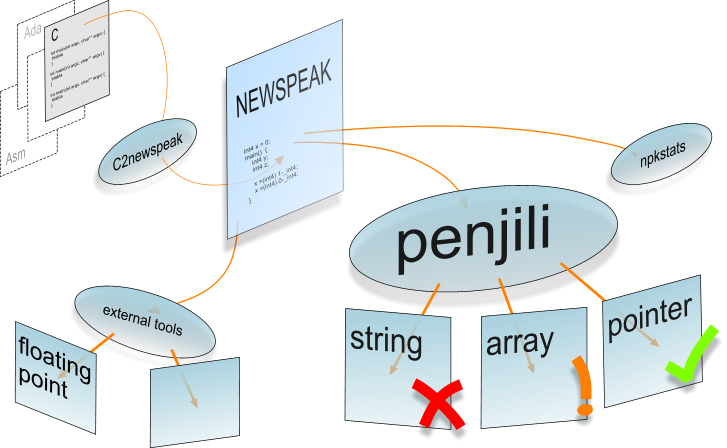
\includegraphics[scale=.5]{img/penjili.png}
\end{frame}

\begin{frame}{Le langage intermédiaire \newspeak}

Un langage adapté à l'analyse statique:

\begin{itemize}
\item simple: il contient peu de constructions
\item explicite: les effets de bords sont explicites
\item expressif: tout programme C peut être converti en \newspeak
\end{itemize}

\end{frame}

\begin{frame}[fragile]{Exemple}

\begin{SaveVerbatim}{compilnpk}
int32 x;
x =(int32) 0;
do {
    while (1) {
        choose {
            -->
                guard((10 > x_int32));
            -->
                guard(! (10 > x_int32));
                goto lbl1;
        }
        x =(int32) coerce[-2**31,2**31-1]
                        (x_int32 + 1);
    }
} with lbl1: {
}
\end{SaveVerbatim}

{\footnotesize
\begin{minipage}{0.3\linewidth}
\insertcode{npk-while.c}
\end{minipage}
\vrule\hspace{2pt}
\begin{minipage}{0.6\linewidth}
\BUseVerbatim{compilnpk}
\end{minipage}
}

\end{frame}

\begin{frame}{Compilation \& analyse}

\begin{tikzpicture}\shorthandoff{!}
\tikzstyle{file}=[draw, shape=rectangle, node distance=2.2cm, minimum
height=1cm, shade, top color=white,
    bottom color=blue!50!black!20, draw=blue!40!black!60, very thick];

\node [file] (c1) {\textcolor{black}{.c}};
\node [file, below of=c1] (c2) {\textcolor{black}{.c}};
\node [node distance=2.2cm, below of=c2] (c3) {};

\node [file, minimum height=0, node distance=5mm, above of=c3,draw] (c3b) {.adb};
\node [file, minimum height=0, node distance=5mm, below of=c3,draw] (c3s) {.ads};

\path (c3b.north west) ++(-3mm,3mm) [draw,dotted] rectangle ($(c3s.south east)+(3mm,-3mm)$);

\node [below of=c3, node distance=2.2cm] (c4){};

\node [file, right of=c1] (cc1) {\textcolor{black}{.c}};
\node [file, right of=c2] (cc2) {\textcolor{black}{.c}};
\node [node distance=2.2cm, right of=c3] (cc3) {};

\node [below of=cc3, node distance=2.2cm](cc4){};

\draw[->] (c1) -- node[above] {{\tiny \ttfamily cpp}} (cc1);
\draw[->] (c2) -- (cc2);

\node [file, right of=cc1] (no1) {\textcolor{black}{.no}};
\node [file, right of=cc2] (no2) {\textcolor{black}{.no}};
\node [file, right of=cc3] (no3) {\textcolor{black}{.no}};

\node [below of=no3, node distance=2.2cm](no4){};

\draw[->] (cc1) -- node[above] {{\tiny \ttfamily c2newspeak -c}} (no1);
\draw[->] (cc2) --  (no2);

\draw[->] ($ (c3b.north east)!0.5!(c3s.south east) + (3mm,0) $) -- node[above] {\tiny \ttfamily ada2newspeak -c} (no3);


\node [file, right of=no2] (npk) {\textcolor{black}{.npk}};

\node [right of=no3, node distance=2.2cm](npk2){};
\node [right of=no4, node distance=2.2cm](npk3){};

\node[draw, ellipse, right of=no2, minimum height=3cm]{};

\draw[->] (no1) -- node {} (npk);
\draw[->] (no2) -- node[above] {{\tiny \ttfamily c2newspeak}} (npk);
\draw[->] (no3) -- node {} (npk);


\node [file, right of=npk, node distance=3cm, yshift=1cm](warn)
    {\textcolor{black}{\parbox{2cm}{\centering Programme \linebreak typé}}};
\node [right of=npk, node distance=3cm, yshift=-1cm](warnn)
    {\textcolor{black}{Erreurs}};

\node [right of=npk3, node distance=3cm](analyser2){};

\node [right of=npk, node distance=3cm] {\small ou};

\draw[->] (npk) -- node[above, yshift=2mm] {{\tiny \ttfamily ptrtype}} (warn);

\draw[->] (npk) -- (warnn);

\draw[->] (c4)   -- node[above, text depth=3pt] {\footnotesize Pr\'etraitement} (cc4);
\draw[->] (cc4)  -- node[above, text depth=3pt] {\footnotesize Compilation} (no4);
\draw[->] (no4)  -- node[above, text depth=3pt] {\footnotesize \'Edition de liens} (npk3);
\draw[->] (npk3) -- node[above, text depth=3pt] {\footnotesize Analyse} (analyser2);
\end{tikzpicture}


% TODO en fait, penjili

\end{frame}

